%!TEX root = ./report.tex
\section{Solution}
The final product combines several technologies to attain an extendable solution with two reusable Xtend workflows at its core. The setup allows the user to edit a sub domain of IFC in a generated Eclipse editor in between the two workflows and saving the edited subset back to the main model on the BIMServer.
\paragraph{}
Design decisions we faced when making this setup. List a bunch of requirements that we can reference in the next section: 
Extracting subset on server og client?
Using BIMServer library ecore metamodel or using XSD generated ecore metamodel
How is the subset defined? MVD could have been used, but we chose not to.
Which model2model tool to use? ATL, QVT, Xtend?

\begin{figure}[htbp]
    \centering
        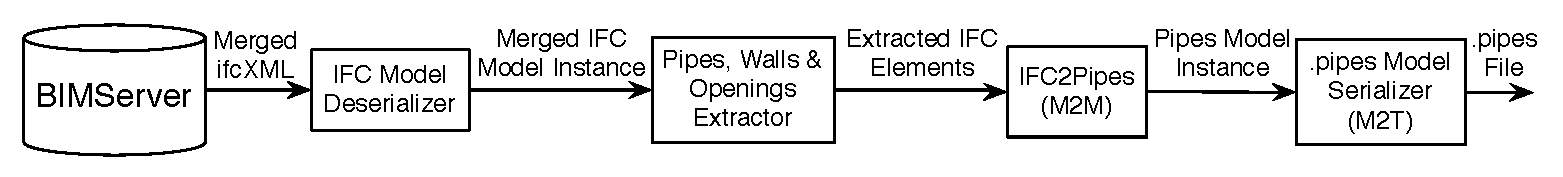
\includegraphics[width=120mm]{images/IFC2Pipes.pdf}
    \caption{IFC to Pipes DSL workflow}
    \label{fig:IFC2PipesWorkflow}
\end{figure}


\begin{figure}[htbp]
    \centering
        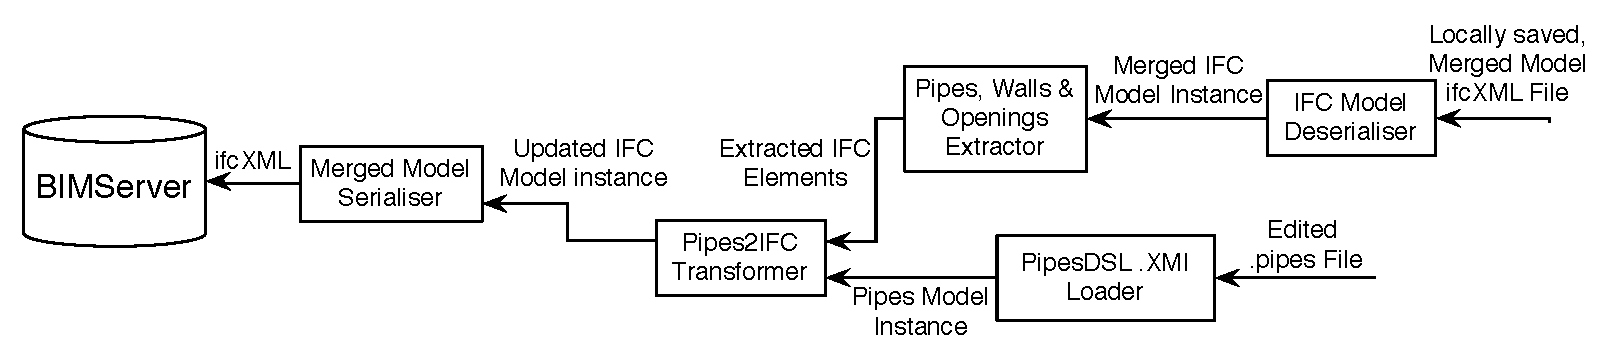
\includegraphics[width=120mm]{images/Pipes2IFC.pdf}
    \caption{Pipes DSL to IFC workflow}
    \label{fig:Pipes2IFCWorkflow}
\end{figure}